\chapter{Krav}
\begin{figure}[h]
\centering 
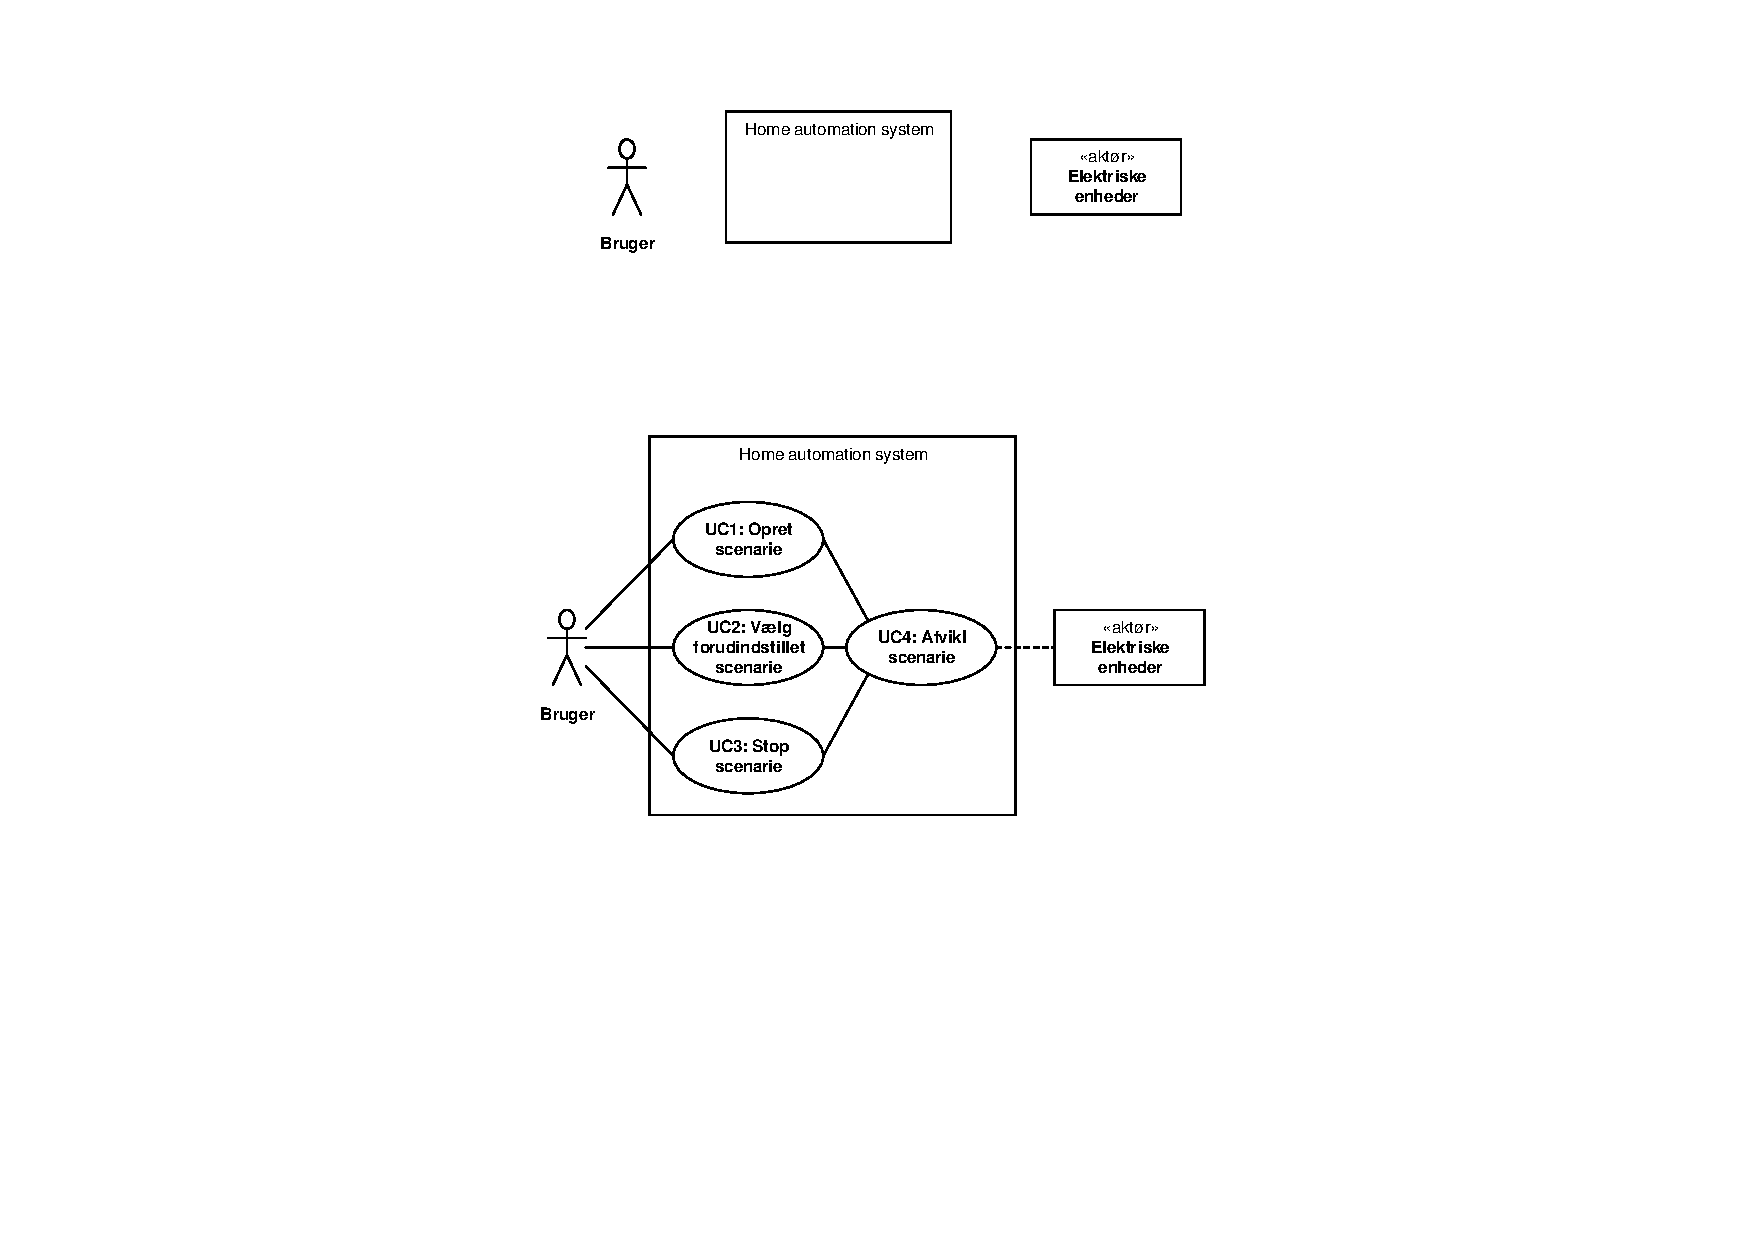
\includegraphics[width=\textwidth, trim=190 200 230 200, clip=true] {../Projektdokumentation/Kravspecifikation/actor.pdf}
\caption{Use Case diagram}
\label{UC diagram}
\end{figure}
De funktionelle krav for systemet er detaljeret beskrevet under \textit{Funktionelle krav} på side \pageref{P-FunkKrav} i dokumentationen, men Use Cases i Figur \ref{UC diagram} diagram giver et overordnet overblik. 

\begin{itemize}
\item UC1: Opret Scenarie 

Giver brugeren mulighed for at oprette et brugerdefineret scenarie, som derefter kan afvikles i systemet (UC4: Afvikl Scenarie). Et scenarie kan indeholde op til 20 aktioner, der hver især udfører en handling (tænd, sluk etc.) for en enhed (lamper, radio, TV) på et tidspunkt fastsat af brugeren. Et brugerdefineret scenarie gemmes som nævnt ikke til senere brug, men eksisterer på transmitter controlleren så længe det er under afvikling. 

\item UC2: Vælg Forudindstillet Scenarie 

Giver brugeren mulighed for at vælge et af tre forudprogrammerede scenarier. Disse tre scenarier ligger i PC-softwaren, og sendes til transmitter controlleren hver gang de skal afvikles (UC4).

\item UC3: Stop Scenarie 

Giver brugeren mulighed for at stoppe et igangværende brugerdefineret eller forudindstillet scenarie. Når brugeren vælger at stoppe et scenarie, slukkes alle tilkoblede enheder.  

\item UC4: Afvikl Scenarie 

Brugeren kan ikke interagere direkte med denne use case. Han kan initiere denne use case indirekte via UC1 eller UC2, og han kan stoppe den indirekte via UC3. 
\end{itemize}

Der er desuden formuleret en række ikke-funktionelle krav, som medvirker til sikring af systemets kvalitet og opfyldelse af projektets afgrænsninger. Disse er nærmere beskrevet i afsnittet \textit{Ikke Funktionelle Krav} på side \pageref{P-ikkeFunkKrav} i projektdokumentetionen.
\clearpage